\documentclass[a4paper, 11pt]{article}
\usepackage[english]{babel}
\usepackage{appendix}
\input{"/media/alessandro/OS/Users/ale57/Documents/1. universita'/ANNO IV (2019-2020)/second semester/header.tex"}

\begin{document}

\title{NNDL: Homework 2 \\ Unsupervised Deep Learning}
\author{Alessandro Lovo}
\maketitle

\section{Introduction}
  This homework will deal with unsupervised deep learning applied to the MNIST dataset of handwritten digits. The focus will be on different architectures of convolutional autoencoders for both classification and image generation problems. In the end also Generative Adversarial Networks (GAN) will be tested.

  \subsection{General framework}
  Network architectures and training procedures rely on a framework of python classes that unfolds as follows:
  \begin{itemize}
    \item \textbf{Encoder}: class inheriting from \emph{torch.nn.Module} that contains the specific architecture of the first part of the autoencoder: it consists in a block of convolutional layers followed by one of fully connected layers. It receives as input a 28 by 28 pixels gray scale image and outputs $N_{latent}$ real numbers.
    \item \textbf{Decoder}: counterpart of the encoder: it takes as input $N_{latent}$ real numbers, passes them through a block of linear layers and one of transposed convolutional layers outputting a 28 by 28 gray scale image.
    \item \textbf{Evolver}: class for handling the training and validation of a general list of concatenated networks, in particular here the list is an \emph{Encoder} followed by a \emph{Decoder}. In this class there is a check at the end of every training epoch to interrupt the learning process. To implement early stopping one just needs to inherit from the \emph{Evolver} class and specify that check condition. In particular the learning process stops if the validation loss isn't decreasing after \emph{patience} number of epochs.
    \item \textbf{KFoldCrossValidator}: class for performing k fold cross validation on a particular set of hyperparameters.
  \end{itemize}


\section{Convolutional autoencoders}
  For simplicity I restricted the hyperparameter space to symmetric autoencoders, i.e. the decoder is a 'mirrored' version of the encoder. For this reason I will point out only the encoder hyperparameters.
  \subsection{Basic solution}
    The structure of this autoencoder is very similar to the one seen in the Lab practices: 3 convolutional layers with number of channels [8, 16, 32], kernel sizes of 3, strides of 2, paddings [1, 1, 0]; then 2 linear layers with 128 and 16 neurons and finally an output layer with $N_{latent} = 4$ neurons. The activation functions between all layers are ReLU and this architecture is trained for 100 epochs with the Adam optimizer with learning rate $10^{-3}$ and weight decay $10^{-5}$ with a batch size of 256 and a 80\%-20\% train validation split of the 60000 training samples. The loss function is the mean square error (MSE) between the original and reconstructed image.

    As we can see from fig \ref{fig:basic} there is no definite convergence, as the loss slowly keeps decreasing, moreover training and validation loss are virtually identical, showing there is no overfitting.

    % \begin{figure}
    %   \centering
    %   \subfloat[]{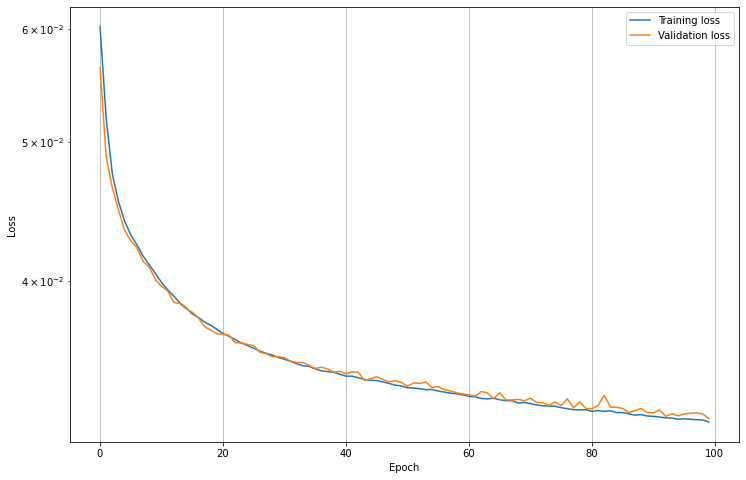
\includegraphics[width=0.4\textwidth]{img/basic_loss.png}} \,
    %   \subfloat[]{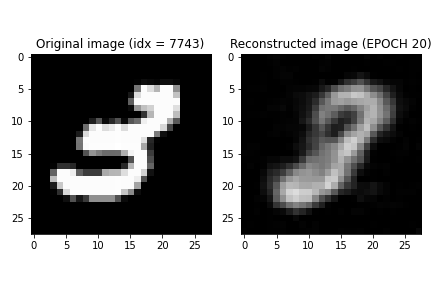
\includegraphics[width=0.4\textwidth]{img/basic/epoch_20.png}} \\
    %   \subfloat[]{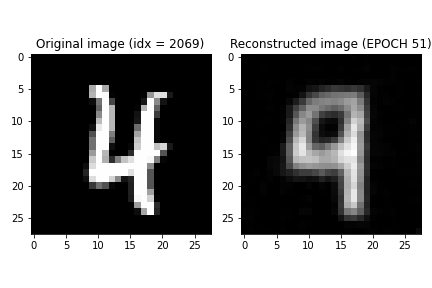
\includegraphics[width=0.4\textwidth]{img/basic/epoch_51.png}} \,
    %   \subfloat[]{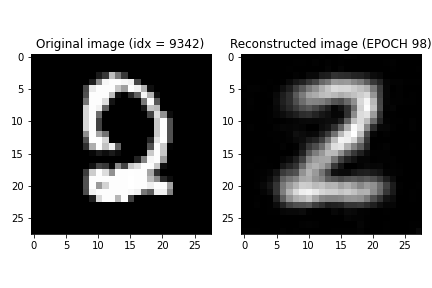
\includegraphics[width=0.4\textwidth]{img/basic/epoch_98.png}}
    %   \caption{Behavior of training and validation loss during learning and some examples of original versus reconstructed images (at epochs 20, 51 and 98).}
    %   \label{fig:basic}
    % \end{figure}

    \begin{figure}
      \centering
      \begin{tabular}{cc}
        \multirow{2}{*}[2.4cm]{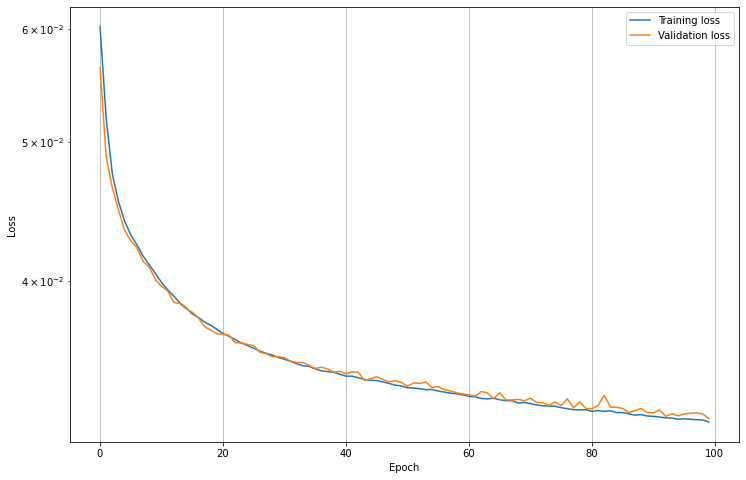
\includegraphics[width=0.55\textwidth]{img/basic_loss.png}}
        & 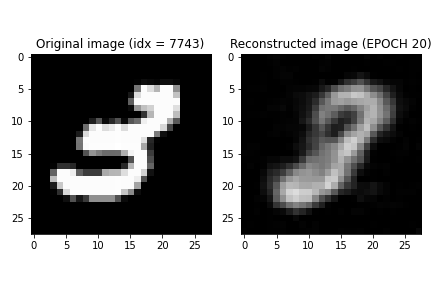
\includegraphics[width=0.3\textwidth]{img/basic/epoch_20.png} \\
        & 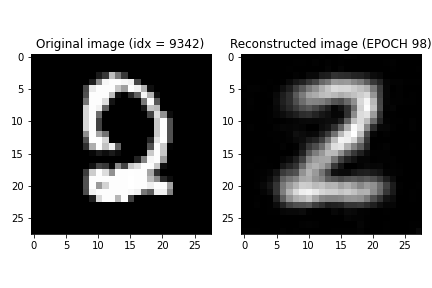
\includegraphics[width=0.3\textwidth]{img/basic/epoch_98.png} \\

      \end{tabular}
      \caption{Behavior of training and validation loss during learning and some examples of original versus reconstructed images (at epochs 20 and 98).}
      \label{fig:basic}
    \end{figure}



  \subsection{More advanced methods}
    In the basic example we witnessed a pretty slow convergence to quite mediocre results: to improve both speed and reconstruction error one needs better architectures and training methods. First of all instead of the MSE loss it is better to use the Binary Cross Entropy (BCE) loss; then I also implemented early stopping, checkpointing the nets back to when the validation loss was at its minimum if after \emph{patience} epochs the validation loss didn't reach a new minimum. At this point I tried more advanced strategies:

    \begin{itemize}
      \item \textbf{Pruning}: every \emph{prune\_every} epochs the \emph{amount} fraction of the weights of the nets that have the lowest L1 norm are set to zero. The \emph{amounts} are potentially different between linear and convolutional layers (usually lower in the latter case) and between decoder and encoder.
      \item \textbf{Dropout}: adding a dropout layer before every hidden linear layer of the nets. Experimenting a bit I found that the nets perform better when dropout is applied only to the encoder.
      \item \textbf{Iterative autoencoding}: up to now we considered only the error between the original image and the first reconstruction. Here I tried to add to the loss also the error between the original image and second and third reconstructions, namely feeding the output of the decoder back to the encoder. However this slowed considerably the training process without yielding considerably better results.
    \end{itemize}

    At this point I proceeded to a hyperparameter search over the following degrees of freedom:
    \begin{itemize}
      \item Number of convolutional layers: 2, 3 or 4
      \item Number of channels: from 4 to $4\cdot2^j$ for the $j^{th}$ convolutional layer
      \item Kernel size: from 2 to 6. Stride: from 1 to 4. Padding: from 0 to half of the kernel size
      \item Number of fully connected hidden layers: 1, 2 or 3
      \item Number of neurons per linear layer: from 8 to $512\cdot2^{-j}$ for the $j^{th}$ layer
      \item Dropout probabilities: from 0 to 0.7
      \item $N_{latent}$: from 1 to 16
      \item Optimizer learning rate (from $10^{-5}$ to $10^{-1}$) and weight decay (from $10^{-7}$ to $10^{-1}$)
      \item train batch size (from 64 to 512) and \emph{patience} for early stopping (from 4 to 16)
      \item \emph{prune\_every}: never or from 1 to 10 and the four pruning \emph{amounts} from 0 to 0.5
    \end{itemize}

    The search was performed with \emph{optuna} at its default setting using a 5 fold cross validation (running only the first two folds and pruning the trials if the validation loss of the first fold was above 0.2) for every hyperparameter combination and adding to the average validation loss a penalty of $10^{-5}$ times the average training time in minutes plus $10^{-2} \cdot N_{latent}$ as further regularizing terms.

    After 60 trials, half of which were pruned, the best hyperparameters are 3 convoultional layers with channels [6,12,17], kernel sizes [2,2,3], strides [1,1,3], paddings [1,0,1]; a single hidden linear layer with 57 neurons after a dropout layer with probability 0.1905 and $N_{latent} = 6$; trained with learning rate of $2.89\cdot10^{-3}$, weight decay of $6.51\cdot10{-7}$, patience of 13 and train batch size of 383. The net was pruned every 5 epochs with amounts [0.398, 0.1, 0.214, 0.068], respectively for encoder linear layers, encoder convolutional layers, decoder linear layers and decoder convolutional layers.

    The best net is then obtained by training with these hyperparameters in a 5 fold setup and choosing the one with the smallest validation loss (0.1253).

    \begin{figure}
      \centering
      \begin{tabular}{cc}
        \multirow{2}{*}[2.4cm]{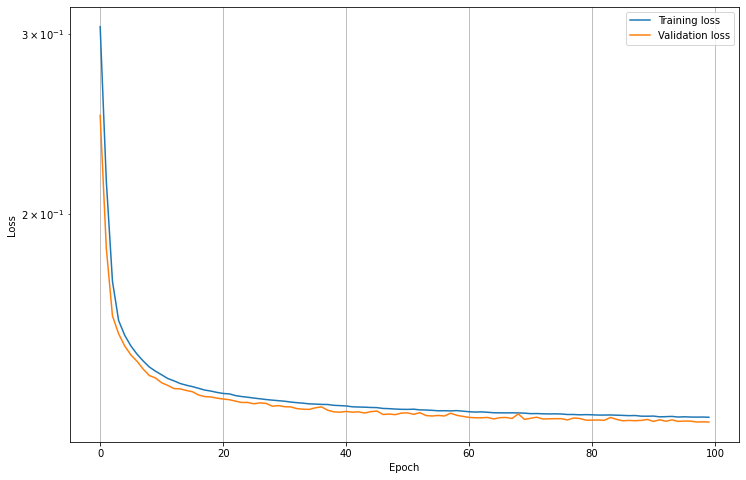
\includegraphics[width=0.55\textwidth]{img/best_loss.png}}
        & 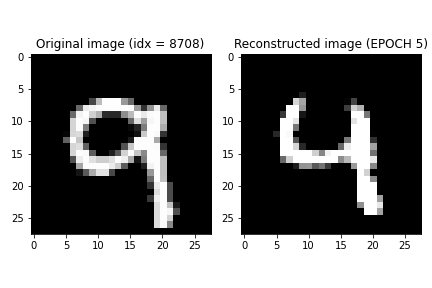
\includegraphics[width=0.3\textwidth]{img/best/epoch_5.png} \\
        & 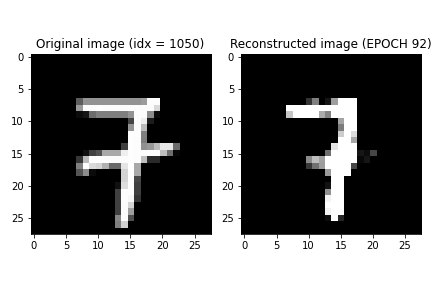
\includegraphics[width=0.3\textwidth]{img/best/epoch_92.png} \\
      \end{tabular}
      \caption{Behavior of training and validation loss during learning of the best net and some examples of original versus reconstructed images (at epochs 5 and 92). Thanks to the BCE loss the reconstructed images are far less blurred than the ones of the basic autoencoder.}
      \label{fig:best}
    \end{figure}

  \subsection{Denoising autoencoder}
    An interesting subset of autoencoders is the one of denoising autoencoders, where the encoder is provided a noisy image and the goal is reconstructing the original image. To add noise to the images one can simply act on the \emph{transform} attribute of the dataset; in particular I tried the following types of noise:

    \begin{itemize}
      \item \textbf{UniformRandomNoise}(\emph{amount}): every pixel value (that ranges from 0 (black) to 1 (white)) is summed to a random number sampled from the uniform distribution between -\emph{amount}/2 and \emph{amount}/2. The pixel values are then clipped to be between 0 and 1.
      \item \textbf{SaltNPepper}(\emph{amount}): \emph{amount} of the pixels of the image are randomly set to 0 or 1.
      \item \textbf{RandomHole}(\emph{size}): a rectangle of size \emph{size} is randomly placed above the image setting to 0 the pixels lying beneath.
      \item \textbf{RandomRotation}(\emph{degrees}): the image is rotated by a random angle sampled from the uniform distribution between -\emph{degrees} and \emph{degrees}.
    \end{itemize}

    Now: in the MNIST dataset digits already appear with different orientations (expecially the digit 1), so it is virtually impossible for the net to discriminate between an 'intrinsic rotation' and a RandomRotation. Also, the RandomHole doesn't produce very interesting results, so I focused on the first two types of noise.

    To deal with noise I started from the pretrained best net previously found (leaving all weights free to be updated) and trained and tested it against different types of noise. The training is performed using the best combination of hyperparameters found before, yielding the results shown in tab \ref{tab:denoising_loss}
    \begin{table}[H]
      \centering
      \begin{tabular}{c|ccccccc}
        \multirow{2}{*}{Trained against} & \multicolumn{3}{c}{Test loss against} \\
          & No noise & SNP(0.1) & URN(0.7) \\
        \midrule
        No additional training & 0.1246 & 0.2459 & 0.3150 \\
        SNP(0.1) (52 epochs) & 0.1239 & 0.1249 & 0.2920 \\
        URN(0.7) (55 epochs) & 0.1233 & 0.2539 & 0.1239 \\
        URN(0.7) + SNP(0.1) (60 epochs) & 0.1236 & 0.1248 & 0.1242 \\
        URN(2) + SNP(0.1) (100 epochs) & 0.1407 & 0.1404 & 0.1403 \\
        \bottomrule
      \end{tabular}
      \caption{Test losses against different types of noise (URN stands for UniformRandomNoise and SNP for SaltNPepper) of the best architecture after different types of training.}
      \label{tab:denoising_loss}
    \end{table}
    \begin{figure}
      \centering
      \subfloat[]{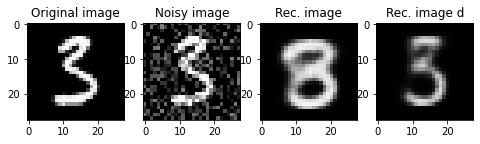
\includegraphics[width=0.4\textwidth]{img/denoising_cfr.png}} \,
      % \subfloat[]{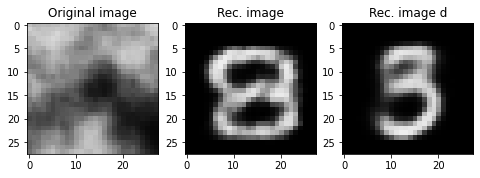
\includegraphics[width=0.4\textwidth]{img/perlin_hallucination.png}} \\
      % \subfloat[]{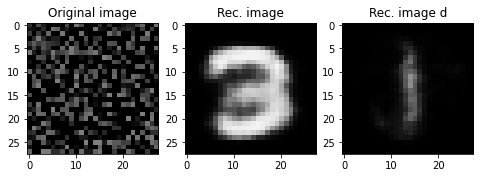
\includegraphics[width=0.4\textwidth]{img/uniform0.7_hallucination.png}} \,
      \subfloat[]{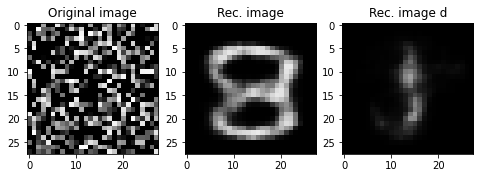
\includegraphics[width=0.4\textwidth]{img/uniform2_hallucination.png}}
      \caption{'Rec image' is the one reconstructed by the best autoencoder with no denoising additional training, while 'Rec image d' is the one reconstructed by the autoencoder trained against URN(2) + SNP(0.1). The denoising autoencoder manages to correctly reconstruct the noisy image, while the simple one fails (a). Also the simple one is more prone to 'hallucinations', i.e. seeing digits in pure noise (b).}
      \label{fig:hallucination}
    \end{figure}

  \vspace{-0.7cm}
  \subsection{Supervised fine-tuning}
    If we take just the pretrained encoder (without denoising) and stack a linear layer with 10 neurons on top of it, we can fine tune some of the weights with supervised learning, obtaining a classifier. To do so I used again the best hperparameters (without pruning), with the exception of the loss function, which now is the Cross Entropy Loss. I tried letting the gradient propagate up different depths in the pretrained encoder, testing every choice in a 5 fold setup. The results are in tab \ref{tab:sup_ft}, where there is an evident jump in performance once we allow some hidden layers of the encoder to be updated.
    \begin{table}[H]
      \centering
      \begin{tabular}{c|ccccccc}
        Deepest non frozen layer & Average train loss & Average validation loss & Average test accuracy \\
        \midrule
        Classifying layer (10 neurons) & 0.3417 & 0.3237 & 0.9126 \\
        Encoder out layer (6 neurons) & 0.2108 & 0.1912 & 0.9452 \\
        Encoder hidden linear layer & 0.0309 & 0.0466 & 0.9862 \\
        Encoder last conv. layer & 0.0206 & 0.0427 & 0.9874 \\
        \midrule
        best net of homework 1 & 0.1062 & 0.0527 & 0.9873 \\
        % \bottomrule
      \end{tabular}
      \caption{The test accuracy is computed as the fraction of correctly classified samples; 'average' means over the 5 folds.}
      \label{tab:sup_ft}
    \end{table}

  \subsection{Visualization techniques}
    There are several ways to visualize the latent space of the encoder: I tried taking a 2D slice of said space, applying PCA and TSNE. Of all these techniques the latter proved to be the most interesting. In fig \ref{fig:tsne} one can appreciate how much the supervised fine tuning helped correctly clusterizing the digits together. On the other hand, to visualize the encoder I made a simple interface to interactively generate images by setting the values of the latent space variables. I recorded the screen of me using it on the basic and best autoencoders: the videos are \url{code/interactive_generation_basic.mp4} and \url{code/interactive_generation_best.mp4}. For the latter, being the latent space six dimensional it is more tricky to obtain meaningful images.

    \begin{figure}
      \centering
      \subfloat[basic encoder]{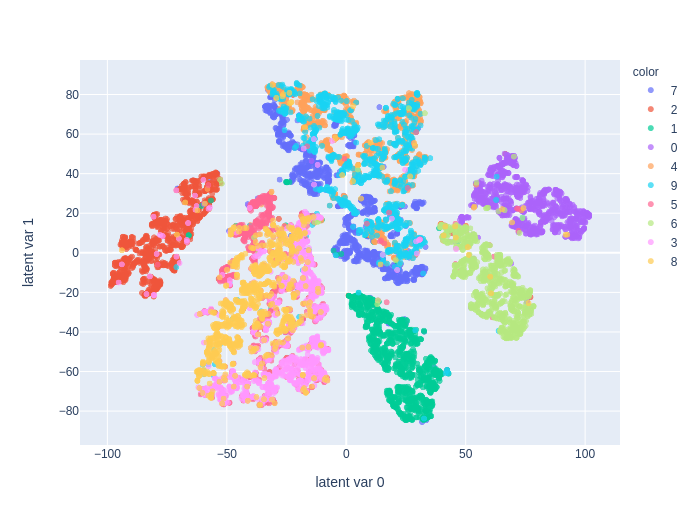
\includegraphics[width=0.4\textwidth]{img/basic_tsne.png}} \,
      \subfloat[best encoder]{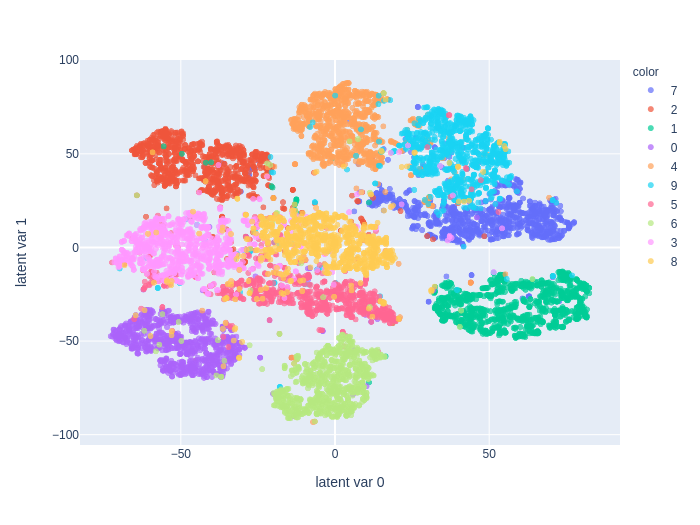
\includegraphics[width=0.4\textwidth]{img/best_tsne.png}} \\
      \vspace{-0.4cm}
      \subfloat[denoising encoder]{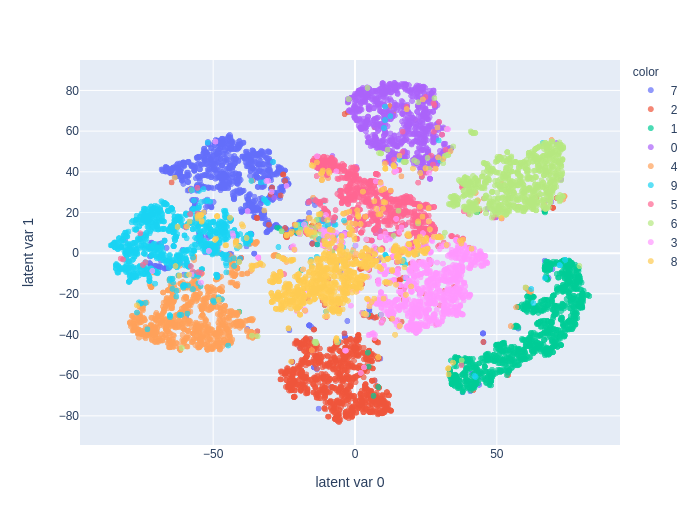
\includegraphics[width=0.4\textwidth]{img/denoising_tsne.png}} \,
      \subfloat[fine-tuned encoder]{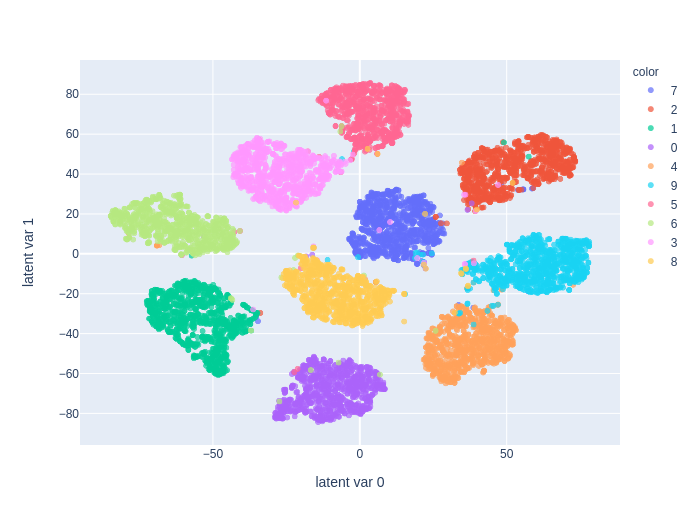
\includegraphics[width=0.4\textwidth]{img/fine-tuned_tsne.png}}
      \caption{2 components TSNE representation of the latent space of different nets.}
      \label{fig:tsne}
    \end{figure}


\section{GAN}
  I tried different types of Generative Adversarial Networks, using slight variations of the best encoder and decoder architectures respectively for the discriminator and generator. In every case real data have a real label and fake images a fake one: the discriminator is trained to correctly distinguish between the two, while the generator descends the gradient of the loss of the discriminator once provided generated fake images, but this time with the real label. Also in every case I implemented the possibility of updating generator and discriminator respectively every $u_g, u_d$ batches, in order to properly synchronize the training and try to avoid bad equilibria.
  \begin{itemize}
    \item \textbf{Simple GAN}: the discriminator has a single output neuron followed by a sigmoid: fake data (produced by the generator starting from gaussian noise on the latent neurons) are labeled with 0 and real ones with 1 and the loss function is the Binary Cross Entropy.
    \item \textbf{Wasserstein GAN (WGAN)}: instead of classifying the images, the discriminator scores them with a real number that is higher the more real it thinks the image is. Real images have a label +1 and fake ones -1; the loss is $l = -\frac{1}{N}\sum_{i=1}^N label_i\cdot score_i$. Moreover at every step of training the weights of the discriminator are clipped, otherwise the it will quickly converge to a bad equilibrium in which it gives scores of the order of $10^7$ and learning stops.
    \item \textbf{Auxiliary Classifier GAN (ACGAN)}: The discriminator has 11 output neurons corresponding to the classes [0, 1, 2, 3, 4, 5, 6, 7, 8, 9, fake] (real images are labeled from 0 to 9 and fake ones as fake) and is trained with the Cross Entropy Loss. The generator has an initial embedding layer taking as input one of the valid labels, then a gaussian noise is summed to the output of the embedding layer to provide variability and the result is fed to the first linear layer of the generator. With this architecture the generator is forced to learn to produce every digit.
  \end{itemize}

  The first two types of GAN were incredibly difficult to train and yielded very bad results (generated images hardly ever resembled digits). On the other hand the ACGAN was able to produce something good. I think this is due to the fact that in the first cases the discriminator has simply to distinguish between real and fake images, and this is a too easy task given the terrible output of the generator; at this point the gradient vanishes when updating the generator and so learning stops. On the other hand in the ACGAN the discriminator has also to discriminate between the real 10 classes of digits and so it doesn't stop learning immediately. Anyways, even in this case the quality of the generated images is pretty low, but most importantly there is virtually no variability in the images, exhibiting a sort of mode collapse.

  \begin{figure}
    \centering
    \subfloat[]{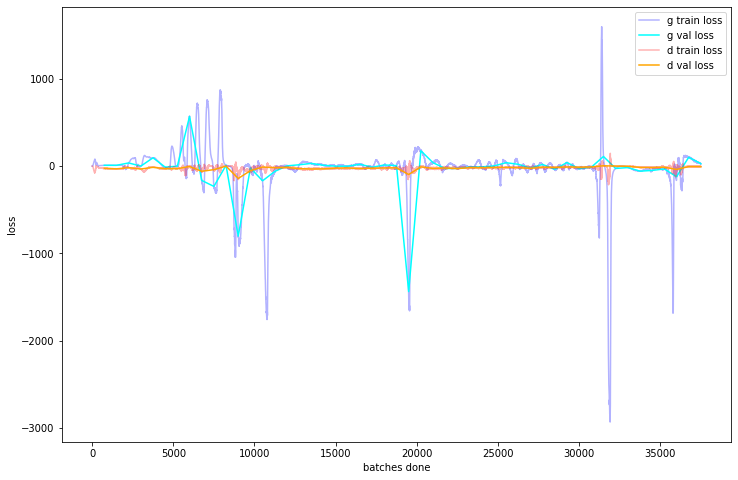
\includegraphics[width=0.45\textwidth]{img/wgan_loss3.png}} \quad
    \subfloat[]{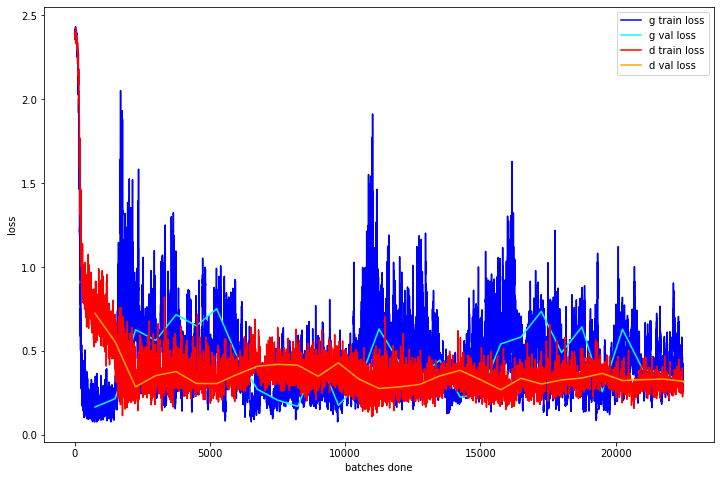
\includegraphics[width=0.45\textwidth]{img/acgan_auto_sync_loss.png}} \\
    \subfloat[]{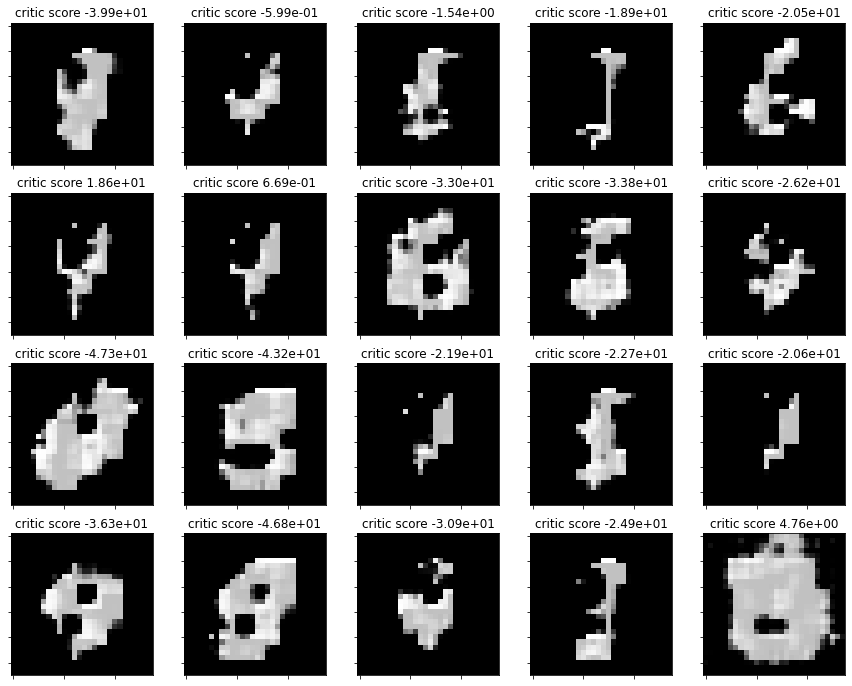
\includegraphics[width=0.3\textwidth]{img/wgan_generation3.png}} \quad
    \subfloat[]{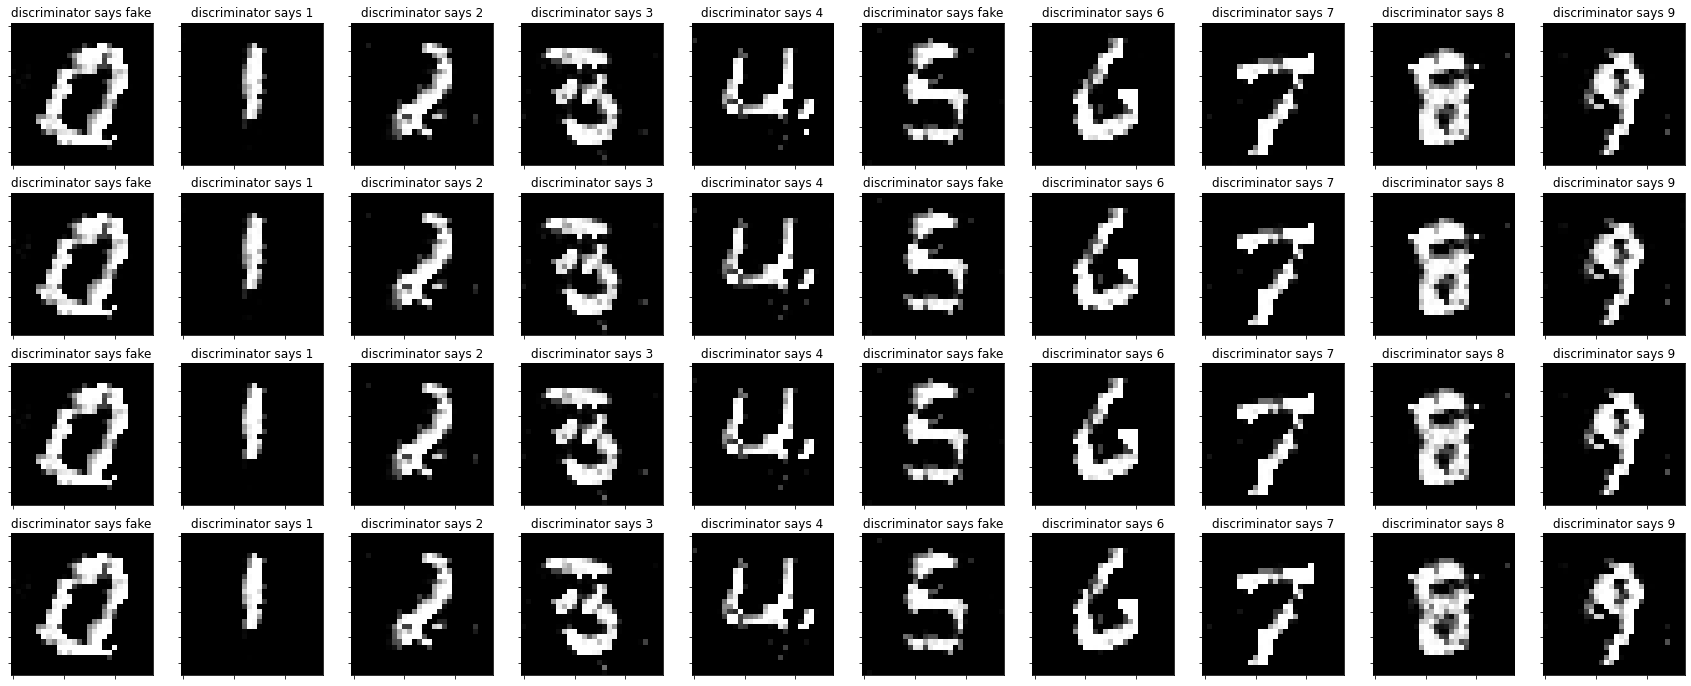
\includegraphics[width=0.6\textwidth]{img/acgan_auto_sync_generation.png}}
    \caption{Losses for generator and discriminator and some generated images for a WGAN (a, c) with $u_g = 5, u_d = 1$ and an ACGAN (b, d) where $u_g, u_d$ are actively tuned during training with a feedback system in order to keep the losses of generator and discriminator as close as possible. On top of the WGAN generated images there is the score given by the discriminator, while for the ACGAN the class assigned by the discriminator; in particular we can see that the generator managed to fool the discriminator for every digit apart 0 and 5, which anyways look reasonable.}
    \label{fig:GAN}
  \end{figure}


















\end{document}
